
%!TEX ROOT=ctutest.tex

\chapter{Identifikace systému}

U robotického manipulátoru zpravidla nejsou zcela známy informace o dynamických parametrech robota, jako jsou momenty setrvačnosti, hmotnosti nebo koeficienty tření jednotlivých os. Tyto informace nejsou v běžných situacích poskytovány ani samotnými výrobci robotů. Je to hlavně proto, že pro zákazníka nejsou tyto údaje důležité, protože se robotické manipulátory dodávají jako hotové uzavřené systémy připravené k použití a jejich řízení je již výrobcem implementováno v jejich řídícím systému.

\section{Způsoby identifikace}

Protože zpravidla nejsou známy všechny dynamické parametry, je pro vytvoření dynamického modelu nutné tyto parametry nějakým způsobem získat nebo odvodit. Toho je možné docílit několika hlavními způsoby.

\subsection{Z přímého měření součástí robota}

Dynamické parametry je možné určit rozebráním robota na menší součásti a přímým měřením jejich dynamických vlastností. Tento způsob se jeví jako nejpřirozenější.

Určení parametrů takovýmto způsobem je ale možné pouze u jednoduchých laboratorních modelů robota tvořených malým počtem součástí. U větších a složitějších robotů jako jsou průmyslové manipulátory je tento způsob náročný časově i způsobem provedení. Jednotlivá ramena sestávají z více komponent, jako jsou samotné kostry ramen, převodovky motorů, napájecí a komunikační vedení motorů atd. Ty mohou dále sestávat z dalších součástek. Rozebrání robota navíc může způsobit ztrátu podpory a záruky ze strany výrobce.

Další nevýhodou je nemožnost zobecnění tohoto způsobu na více typů robotů. Každý typ robota by se musel rozebrat a změřit, i kdyby se jednalo o robota podobného typu a konstrukce. Proto se tato práce tímto postupem dále nezabývá.    

\subsection{Z 3D modelu}

Výrobci často poskytují ke stažení 3D modely svých robotů. Ty je možné analyzovat v nástrojích CAD jako je například AutoCAD nebo Siemens NX, které jsou schopny počítat momenty setrvačnosti a hmotnosti libovolně složitých objektů. Výhodou tohoto postupu je jeho rychlost a jednoduchost. Navíc je takto možné získat požadované parametry i bez nutnosti přístupu k opravdovému fyzickému robotu. Tento postup je také možné zobecnit na libovolný typ robota. Stačí k němu jen mít jeho odpovídající 3D model. 3D model robota KUKA KR5 Arc v prostředí Siemens NX 10.0 je na obrázku \ref{kuka_3d_pic}.

\begin{figure}[ht]
    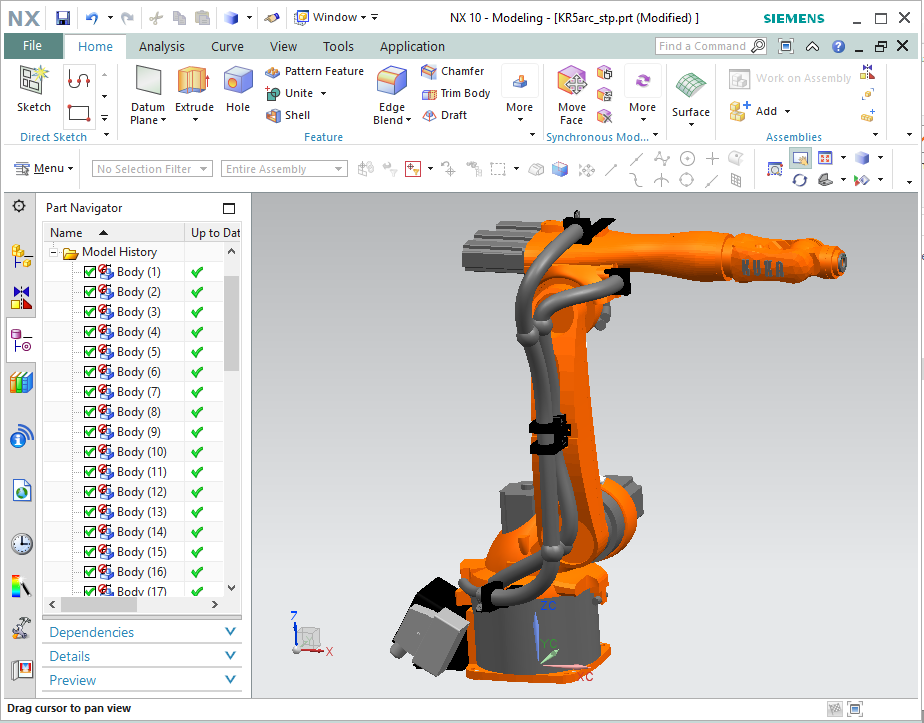
\includegraphics[width=0.8\textwidth]{kuka_3d}
    \caption{3D model robota KUKA KR5 Arc v prostředí Siemens NX 10.0.}
    \label{kuka_3d_pic}
\end{figure}

3D model ale zpravidla popisuje pouze povrchovou geometrii jednotlivých komponent robota a neobsahuje informace o jejich vnitřní konstrukci ani typu použitých materiálů, jejich skutečné hmotnosti nebo jejich hustoty. Je sice možné považovat jednotlivá ramena robota za homogenní a hmotnost odhadnout z celkové hmotnosti robota udávané v jeho datasheetu, tento postup ale dává jen velmi hrubý odhad dynamických parametrů. 

Navíc z 3D modelu není možné získat informace o koeficientech tření v jednotlivých osách. Tento postup je zde použit pouze pro účely porovnání určených hodnot.
\label{z_3d_modelu_sec}

\subsection{Z rovnic}
\label{z_rovnic_sec}
Neznámé dynamické parametry je možné přesně vypočítat pomocí dynamických rovnic robota. 

Přestože jsou dynamické rovnice robota \ref{celkova_dyn_rovnice_eq} nelineární vůči jednotlivým zobecněným souřadnicím, jsou lineární vůči jednotlivým složkám dynamických parametrů [\cite{}][\cite{}]. Proto je tyto rovnice možné je přepsat do tvaru

\begin{equation}
T(t) = H(\ddot{\theta}(t),\dot{\theta}(t),\theta(t))P
\label{eq_lin_par}
\end{equation}
kde
\begin{description}
\item[$T(t) = {\big[T_1(t)  \dotsm  T_n(t)\big]}^{T}$] je vektor momentů sil na osách v čase $t$ 
\item[$P = {\big[P_1  \dotsm  P_n\big]}^{T}$] je vektor neznámých dyn. parametrů jednotlivých os
\item[$n$] je počet os
\end{description} \noindent
a \ \ \ \ \ \ $P_i = {\big[I_{ixx} \ I_{ixy} \ I_{iyy} \ I_{iyz} \ I_{izz} \ I_{izx} \ m_i \ m_id_{ix} \ m_id_{iy} \ m_id_{iz} \ f_{vi} \ f_{ci}\big]}^{T}$ \\
\\
\\
kde
\noindent
\begin{description}
\item[$I_{ijk}$] je složka setrvačnosti pro link $i$ vůči souřadnicím $j$ a $k$
\item[$r_{ij}$] je složka vektoru těžiště linku $i$ vyjádřená v souřadnici $j$
\item[$m_{i}$] je hmotnost linku $i$
\item[$f_{vi}$] je koeficient viskózního tření linku $i$
\item[$f_{ci}$] je koeficient Coulombova tření linku $i$
\end{description}

Neznámých parametrů pro jedno rameno odpovídá počtu složek vektoru $P_i$. Ten je roven 12. U průmyslového manipulátoru se šesti rotačními osami je tedy neznámých parametrů celkem 72. 

Počet neznámých parametrů je možné zredukovat. Je to dáno tím, že některé parametry dynamiku robota neovlivní. Důvodem je to, že se některé linky mohou otáčet pouze kolem některé z os. Příkladem může být osa 1 (spojená se zemí, viz schéma \ref{kuka_kr5_axes_pic}), která se v prostoru může otáčet jen kolem vertikální osy. Tím je možné zanedbat momenty setrvačnosti mimo tuto vertikální osu a také její hmotnost a polohu jejího těžiště. Zároveň je možné si model zjednodušit uvažováním pouze prvků na hlavní diagonále tenzorů setrvačnosti a zanedbáním prvků mimo ni.

Díky tomu klesne počet neznámých parametrů v případě šestiosového robota na číslo 48. V následující tabulce (tabulka \ref{tab_hled_param}) je přehled výsledných neznámých dynamických parametrů robota KUKA KR5 Arc.
\\

\begin{table}[ht]
  \centering
  \caption{Tabulka nezámých parametrů robota KUKA KR5 Arc.}
    \begin{tabular}{c|lllllllll}
    \multicolumn{1}{c|}{Osa} & \multicolumn{9}{c}{Neznámé parametry}  \\
    \hline
    1 &       	  &	          & $I_{1zz}$ &          &          &          & & $f_{v1}$ & $f_{c1}$ \\
    2 & $I_{2xx}$ & $I_{2yy}$ & $I_{2zz}$ & $d_{2x}$ & $d_{2y}$ & $d_{2z}$ & $m_{2}$ & $f_{v2}$ & $f_{c2}$ \\
    3 & $I_{3xx}$ & $I_{3yy}$ & $I_{3zz}$ & $d_{3x}$ & $d_{3y}$ & $d_{3z}$ & $m_{3}$ & $f_{v3}$ & $f_{c3}$ \\
    4 & $I_{4xx}$ & $I_{4yy}$ & $I_{4zz}$ & $d_{4x}$ & $d_{4y}$ & $d_{4z}$ & $m_{4}$ & $f_{v4}$ & $f_{c4}$ \\
    5 & $I_{5xx}$ & $I_{5yy}$ & $I_{5zz}$ & $d_{5x}$ & $d_{5y}$ & $d_{5z}$ & $m_{5}$ & $f_{v5}$ & $f_{c5}$ \\
    6 & $I_{6xx}$ & $I_{6yy}$ & $I_{6zz}$ & $d_{6x}$ & $d_{6y}$ & $d_{6z}$ & $m_{6}$ & $f_{v6}$ & $f_{c6}$ \\
    \end{tabular}%
  \label{tab_hled_param}%
\end{table}%

Hledané parametry je poté možné vypočítat z rovnice \ref{eq_lin_par} jejich vyjádřením ve tvaru

\begin{equation}
P = H\big(\ddot{\theta}(t),\dot{\theta}(t),\theta(t)\big)^{-1}T(t)
\label{eq_lin_par_inv}
\end{equation}

K výpočtu vektoru $P$ neznámých parametrů je nejprve potřebné vykonat pohyb na robotu po nějaké trajektorii a měřit polohy, úhlové rychlostí, úhlová zrychlení a momenty sil na jednotlivých osách. Do matice $H$ se poté dosadí polohy, úhlové rychlosti a úhlová zrychlení jednotlivých os v čase $t$ a do vektoru $T(t)$ změřené momenty sil v čase $t$. 

Protože je ale neznámých parametrů více než rovnic, nelze tuto rovnici vyřešit jednoznačně. Tento problém lze jednoduše vyřešit naměřením na trajektorii více bodů a jejich následným dosazením do rovnice \ref{eq_lin_par_inv} v různých časech. Důležité je na trajektorii mít tolik bodů, aby z této rovnice vznikla rovnice přeurčená. Takovou rovnici je poté možné řešit například použitím metody nejmenších čtverců, která minimalizuje střední odchylku mezi skutečnými a odhadnutými parametry a navíc je schopna eliminovat vliv šumu měření. 

\subsection{Excitační trajektorie}

Odhadované parametry vypočítané výše popsaným postupem jsou ale silně závislé na zvolené trajektorii, na které jsou měřeny dynamické veličiny. 

Aby se tímto způsobem správně odhadly všechny neznámé parametry, je potřeba s robotem provést pohyby po takové trajektorii, na které by byly vybuzeny všechny dynamické složky robota, tzn. aby se do dynamiky promítly všechny neznámé parametry. Nedostatečně excitující trajektorie sice dá nějaké výsledky, ty budou ale platit pouze pro pohyby po této trajektorii nebo jejím okolí.

Ve vědeckých článcích a v jiných publikacích např. \cite{clos_dyn_par}\cite{dyn_mod_ind}\cite{dyn_ind_mits} se na jednotlivých osách doporučují trajektorie, které je možné popsat konečnou Fourierovou řadou. Jejich výhodou je, že díky vlastnostem harmonické funkce jsou poté jednotlivé polohy, rychlosti i zrychlení rovněž kombinací harmonických průběhů. Tím se maximalizuje vliv hledaných dynamických parametrů a minimalizuje vliv šumu měření. 

Protože se průmyslové manipulátory používají převážně pro polohování, jejich řídící systémy zpravidla neumožňují na osách provádět čistě harmonické průběhy. Řídící systém robota KUKA KR5 Arc umožňuje pouze nastavit sadu požadovaných poloh os, kterých musí osy dosáhnout a rychlosti/zrychlení, s jakými se má tento pohyb vykonat. Z toho důvodu je nutné robotu poskytnout sérii bodů popisujících harmonický průběh. Výsledná trajektorie robota je poté pouze aproximací harmonického průběhu.  


\section{Postup identifikace}

Při identifikaci parametrů robota KUKA KR5 Arc se postupovalo způsobem popsaným výše v sekci \ref{z_rovnic_sec}. 

Pomocí nástroje ReDySim se vygenerovala soustava šesti rovnic dynamiky robota. Protože ReDySim neuvažuje tření na jednotlivých osách, bylo nutné toto tření do vygenerovaných rovnic doplnit ručně. Výsledná soustava rovnic se poté převedla do maticového tvaru lineárního vůči neznámým dynamickým parametrům (rovnice \ref{eq_lin_par}). 

Za vektor $P$ neznámých parametrů byl zvolen vektor s parametry všech šesti os
\[\addtolength{\arraycolsep}{-1.5pt}
\begin{split}
P &= 
[\begin{matrix} I_{1x} & I_{1y} & I_{1z} &\cdots &I_{6x} & I_{6y} & I_{6z} \end{matrix} \\
 &\qquad\qquad \begin{matrix}  m_1 & m_1d_{1x} & m_1d_{1y} & m_1d_{1z} &\cdots & m_6 & m_6d_{6x} & m_6d_{6y} & m_6d_{6z} \end{matrix} \\
 &\qquad\qquad\qquad\qquad \begin{matrix} f_{v1} & f_{c1} &\cdots & f_{v6} & f_{c6} \end{matrix}]^{T}
\end{split}
\]

Do matic $H\big(\ddot{\theta}(t),\dot{\theta}(t),\theta(t)\big)$ a $T(t)$ se dosadily jednotlivé polohy, úhlové rychlosti, úhlová zrychlení a momenty sil naměřené v různých časech na identifikační trajektorii. Vektor neznámých parametrů $P$ se poté vypočítal z rovnice \ref{eq_lin_par_inv} metodou nejmenších čtverců. 

Protože jsou dynamické rovnice robota silně nelineární, může se stát, že řešitel metody nejmenších čtverců nenalezne globálně optimální řešení, ale skončí v některém z lokálních minim. Je také možné, že řešitel nalezne řešení, které bude správně matematicky, fyzikálně ale nebude dávat smysl (záporné hmotnosti ramen, apod.). Z tohoto důvodu je vhodné nějakým způsobem omezit prostor, ve kterém se má řešení hledat.

V této práci byl pro řešení metody nejmenších čtverců v MATLABu použit solver \texttt{lsqlin}, který umožňuje specifikovat hranice, ve kterých se má řešení hledat. První z podmínek bylo, že všechny hmotnosti a momenty setrvačnosti mají mít kladné hodnoty. Dále se nastavilo omezení na hledané polohy těžiště ramen tak, aby tato těžiště neležela mimo fyzický objem ramen. Posledním omezením bylo nastavení přesných hmotností ramen, které se podařilo nalézt ve zdrojových datech robota.

\label{postup_identifikace_ch}

\subsection{Identifikační trajektorie}

Protože je prostor kolem robota omezen, není možné s robotem provádět pohyby v plném rozsahu. Proto bylo nutné tomu identifikační trajektorii přizpůsobit. Identifikační trajektorie byla vytvořena složením několika nezávislých trajektorií. 

V první části se pohybovalo pouze s posledními třemi osami (osa 6, osa 5 a osa 4). Ostatní osy byly v pevně zafixované pozici. Nejprve se opakovaně pohybovalo pouze poslední šestou osou v maximálním možném rozsahu v obou směrech otáčení. K tomu se následně přidal obdobný pohyb páté osy a nakonec se stejným způsobem přidal i pohyb čtvrté osy. Tímto se pokryla maximální možná škála pohybů posledních tří os.

Následovala část pro identifikaci prvních tří os. U těchto os je problém v tom, že osa 2 a osa 3 mají vzájemně rovnoběžné osy otáčení (viz obrázek \ref{kuka_kr5_axes_pic}). Proto je obtížné nezávisle identifikovat některé jejich parametry. Příkladem může být identifikace momentů setrvačnosti vzhledem k osám kolmým na osy jejich rotace. Osou 3 není možné kolem těchto os otáčet, aniž by se zároveň kolem stejné osy neotáčela osa 2 a naopak.    

V tomto případě se postupovalo nejprve hýbáním osou 3 v plném rozsahu a zafixováním os 1 a 2. Následně se zafixovala osa 3 a hýbalo se osou 2. Tímto se pokryly pohyby nezávislé na rotaci kolem osy 1.

Pohyby závislé na rotaci kolem osy 1 se provedly tak, že se nejprve hýbalo s osou 1 s rameny os 2 a 3 pevně zafixovanými ve vertikální poloze. Poté se stejné pohyby provedly s ramenem osy 3 ve vodorovné poloze a následně s oběma rameny (2 a 3) ve vodorovné poloze.

Výsledná identifikační trajektorie byla vytvořena spojením těchto dvou trajektorií v jednu. Nástroj TRACE byl nastaven tak, aby prováděl měření poloh, úhlových rychlostí, úhlových zrychlení, momentů sil a proudů na všech osách. 

\section{Skript pro MATLAB}

Pro účely identifikace robota KUKA KR5 Arc byl vytvořen skript pro použití v MATLABu, který umožňuje vytvoření dynamického modelu, načtení trajektorií, identifikaci parametrů a simulaci výsledků.

Skript je rozdělen na několik po sobě jdoucích podprogramů, které jde spouštět vcelku nebo po jednotlivých částech. Komentáře ve skriptu jsou psány v anglickém jazyce pro případné rozšíření jeho použití.

První část je univerzální pro libovolného robota s rotačními osami. Určují se zde základní parametry robota, jako je počet os, délky jednotlivých ramen, parametry převodovek a počet měřených veličin. Dále se zde zadávají vlastnosti motorů, mezi něž patří momentové konstanty a odpory a indukčnosti vinutí. 

Další část je částečně závislá na použitém robotu. V této části se načítá změřená trajektorie robota. Robot KUKA KR5 Arc používá k měření trajektorií nástroj TRACE. Tento nástroj ukládá data ve speciální struktuře ve formátu .r64. Tu je potřeba rozložit na jednotlivé měřené složky a ty dále vynásobit převodními koeficienty měření. Jiné typy robotů, obzvláště roboti od jiných výrobců budou pravděpodobně mít změřené trajektorie uložené v jiných formátech a jiným způsobem. Proto je potřeba v případě použití jiného robota skript upravit nebo doplnit pro správné načítání těchto dat. Výsledkem této části je matice naměřených trajektorií pro jednotlivé osy a veličiny. 

Následující části jsou již zcela nezávislé a univerzální pro použití pro libovolného robota.  

Nejprve je vytvořen vektor $P$ parametrů v symbolickém tvaru. Následuje načtení vygenerovaných rovnic z nástroje ReDySim, jejich převod do symbolického tvaru a uložení do matice rovnic. Z té je poté vygenerovaná matice $H_i\big(\ddot{\theta}(t),\dot{\theta}(t),\theta(t)\big)$ se symbolickými proměnnými, do kterých je možné dosazovat změřená data.

Postupným dosazováním naměřených bodů na trajektorii (polohy, úhlové rychlosti a úhlová zrychlení) do matice $H_t\big(\ddot{\theta}(t),\dot{\theta}(t),\theta(t)\big)$ je vytvořena matice $H$. Současně je vytvořen vektor $T$ s dosazenými změřenými momenty sil.

Tyto vektory a matice jsou poté předány solveru \texttt{lsqlin}, který vypočte vektor $P$ řešením rovnice \ref{eq_lin_par_inv} metodou nejmenších čtverců. Zároveň je zde možné nastavit horní i spodní hranice jednotlivých parametrů vektoru $P$ ve kterých má solver řešení hledat.

Odvozené parametry je možné v další části hned odsimulovat a porovnat se skutečnými změřenými trajektoriemi.

V poslední části je provedena analýza vlivu odchylek v hodnotách parametrů na přesnost energetického modelu robotu.

\section{****** Vliv odchylek *********}

Vliv odchylek v hodnotách parametrů na přesnost energetického modelu robotu je analyzován pomocí metody Monte Carlo. Ke každému z parametrů je náhodně přičteno 10 hodnot z rozsahu $p \in [-0.25P_i,0.25P_i]$ se kterými je poté provedena simulace a vypočítaná střední odchylka mezi simulací a změřenými průběhy. Následně je vyhodnoceno, při jakých odchylkách parametrů byl největší rozdíl mezi simulovaným a změřeným průběhem.